\documentclass[12pt]{scrartcl}

\usepackage[utf8]{inputenc}
\usepackage[naustrian]{babel}
\usepackage{caption}
\usepackage{graphicx}
\usepackage{verbatim}
\usepackage[T1]{fontenc}
\usepackage{lmodern}
\usepackage{subcaption}
\usepackage{amsmath}
\usepackage{mathtools}
\usepackage{amsfonts} 
\usepackage{algorithm2e}
\usepackage{listings}

%pdfs
\usepackage{pdfpages}
\usepackage{tikz}

%page borders
\usepackage{geometry}
\geometry{left=2.5cm,right=2.5cm,top=3cm,bottom=2.5cm}

\usepackage{minted}
\setminted {
	%style=igor, %borland, autumn, vs
	encoding=utf-8,
	autogobble,
	tabsize=4,
	linenos,
	breaklines,
	keywordcase=upper,
	%escapeinside=||
	%bgcolor=bg
	%frame=single
}
% binary tree
\usepackage{tikz-qtree}

\newenvironment{code}{\captionsetup{type=listing}}{}

%title/footer/header values
\usepackage{titling}
\title{ADF2/PRO2 UE08}
\author{Elias Leonhardsberger}
\date{\today{}, Hagenberg}

%footer/header
%\usepackage[automark]{scrpage2}
%\pagestyle{headings}
%\clearscrheadfoot
%\ihead{\thetitle}
%\chead{\theauthor}
%\ohead{\today}
%\cfoot{Seite \pagemark}

\begin{document}
\clearpage
\thispagestyle{empty}
\begin{tikzpicture}[remember picture, overlay]
	\node at (current page.center) {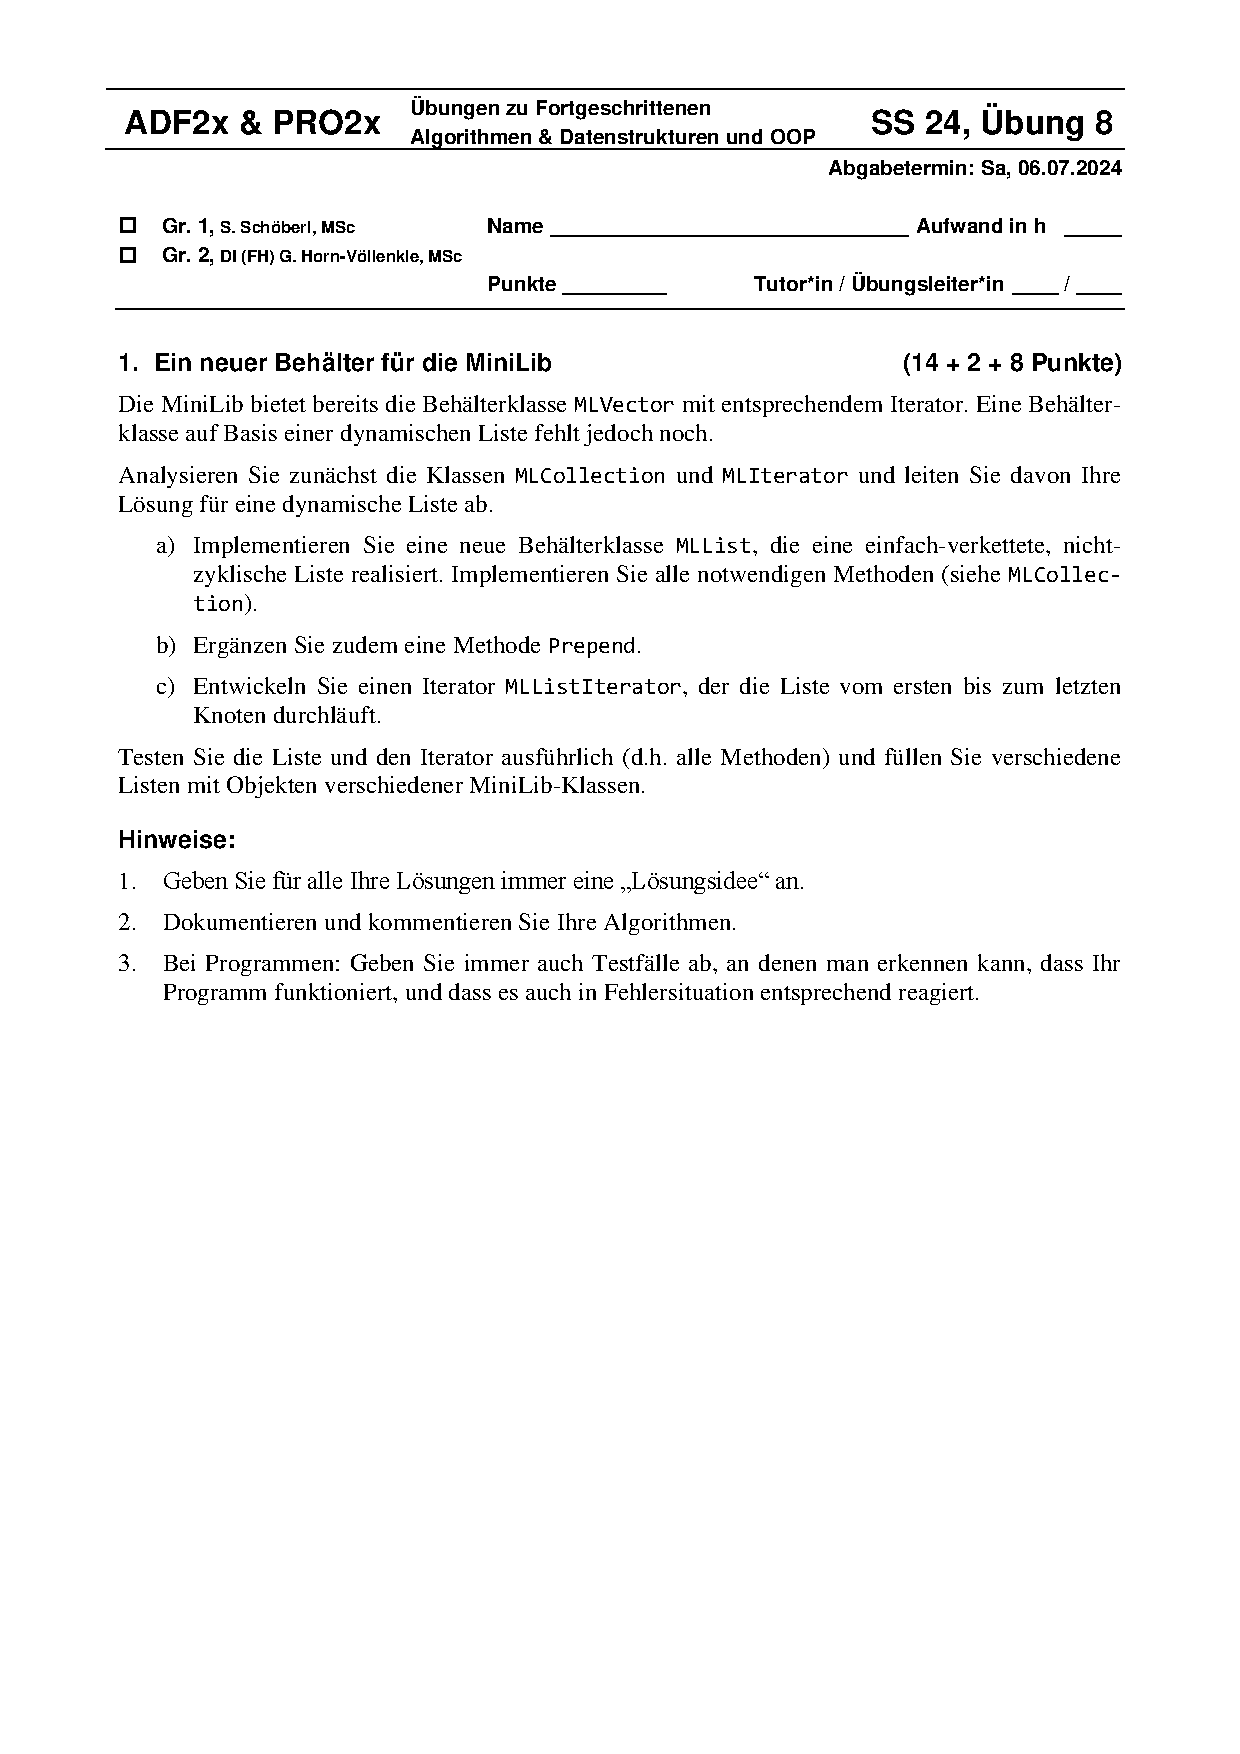
\includegraphics[page=1]{Angabe.pdf}};
	\begin{scope}[shift={(current page.south west)},every node/.style={anchor=base west}]
		\node at (10cm, 25.8cm) {\theauthor};
		\node at (18.2cm, 25.8cm) {3};
		\node at (1.87cm, 25.75cm) {X};
	\end{scope}
\end{tikzpicture}

\maketitle
\tableofcontents

\pagebreak

\section{Ein neuer Behälter für die MiniLib}
\subsection{Lösungsidee}
Die Angabe beschreibt bereits ziemlich genau den Ablauf der Implementierung und außerdem wurden die gefragen Methoden schon bei früheren Übungen gemacht. Die Tests werden wieder wie Unittests umgesetzt.

Der MiniLib Sourcecode, bis auf MLColl.pas, wird nicht in der Abgabe angehängt, da sich kein Code geändert hat. MLColl wird angehängt da es sich hier um die Basisklasse der Liste handelt.
\subsection{Souce Code}
\subsubsection{MLColl.pas}
\inputminted[]{pas}{../../../pascal/PascalWorkspace/UE8/Units/MLColl.pas}
\subsubsection{MLLi.pas}
\inputminted[]{pas}{../../../pascal/PascalWorkspace/UE8/Units/MLLi.pas}
\pagebreak
\subsection{Tests}
\subsubsection{TestMLList.pas}
\inputminted[]{pas}{../../../pascal/PascalWorkspace/UE8/TestMLList.pas}
\pagebreak
\subsection{Testergebnisse}
\begin{figure}[ht]
	\centering
	\includegraphics[width=1\linewidth]{../../../pascal/PascalWorkspace/UE8/TestFiles/Result.png}
	\caption{Ausgabe des Testprogramms \emph{TestMLList}}
\end{figure}
\end{document}